% Options for packages loaded elsewhere
\PassOptionsToPackage{unicode}{hyperref}
\PassOptionsToPackage{hyphens}{url}
%
\documentclass[
]{article}
\usepackage{amsmath,amssymb}
\usepackage{lmodern}
\usepackage{iftex}
\ifPDFTeX
  \usepackage[T1]{fontenc}
  \usepackage[utf8]{inputenc}
  \usepackage{textcomp} % provide euro and other symbols
\else % if luatex or xetex
  \usepackage{unicode-math}
  \defaultfontfeatures{Scale=MatchLowercase}
  \defaultfontfeatures[\rmfamily]{Ligatures=TeX,Scale=1}
\fi
% Use upquote if available, for straight quotes in verbatim environments
\IfFileExists{upquote.sty}{\usepackage{upquote}}{}
\IfFileExists{microtype.sty}{% use microtype if available
  \usepackage[]{microtype}
  \UseMicrotypeSet[protrusion]{basicmath} % disable protrusion for tt fonts
}{}
\makeatletter
\@ifundefined{KOMAClassName}{% if non-KOMA class
  \IfFileExists{parskip.sty}{%
    \usepackage{parskip}
  }{% else
    \setlength{\parindent}{0pt}
    \setlength{\parskip}{6pt plus 2pt minus 1pt}}
}{% if KOMA class
  \KOMAoptions{parskip=half}}
\makeatother
\usepackage{xcolor}
\usepackage{graphicx}
\makeatletter
\def\maxwidth{\ifdim\Gin@nat@width>\linewidth\linewidth\else\Gin@nat@width\fi}
\def\maxheight{\ifdim\Gin@nat@height>\textheight\textheight\else\Gin@nat@height\fi}
\makeatother
% Scale images if necessary, so that they will not overflow the page
% margins by default, and it is still possible to overwrite the defaults
% using explicit options in \includegraphics[width, height, ...]{}
\setkeys{Gin}{width=\maxwidth,height=\maxheight,keepaspectratio}
% Set default figure placement to htbp
\makeatletter
\def\fps@figure{htbp}
\makeatother
\usepackage[normalem]{ulem}
\setlength{\emergencystretch}{3em} % prevent overfull lines
\providecommand{\tightlist}{%
  \setlength{\itemsep}{0pt}\setlength{\parskip}{0pt}}
\setcounter{secnumdepth}{-\maxdimen} % remove section numbering
\ifLuaTeX
  \usepackage{selnolig}  % disable illegal ligatures
\fi
\IfFileExists{bookmark.sty}{\usepackage{bookmark}}{\usepackage{hyperref}}
\IfFileExists{xurl.sty}{\usepackage{xurl}}{} % add URL line breaks if available
\urlstyle{same} % disable monospaced font for URLs
\hypersetup{
  hidelinks,
  pdfcreator={LaTeX via pandoc}}

\author{}
\date{}

\begin{document}

«НЕФОРМАЛЬНАЯ ЛОГИКА И МАТЕМАТИКА»

\textbf{ПРОИЗВОДНАЯ ФУНКЦИИ. ПОНЯТИЕ ПРОИЗВОДНОЙ ФУНКЦИИ}

Толстопятов Алексей А.

\textbf{Определение}: \uline{Производная функции} --- это понятие,
которое используется для определения скорости изменения значения функции
при изменении аргумента.

Другими словами, \uline{производная функции} показывает,
\uline{насколько быстро меняется значение (y) функции} при изменении
аргумента (x).

Знание функций и их производных помогает решать множество задач в
математике и других областях знаний, таких как физика и экономика.

\emph{Необходимость в производных функции возникла в XVII веке в связи с
потребностью вычисления огромного количества задач из математики, физики
и механики. Основными из них были, например, вычисление скорости
прямолинейного неравномерного движения и построение касательной к
произвольной плоской кривой.}

\emph{К открытию дифференциального исчисления пришёл английский учёный
Исаак Ньютон при решении задач о скорости движения материальной точки в
данный момент времени (мгновенной скорости). Он опубликовал свои
результаты в трактате «Метод флюксий и бесконечных рядов» в 1671 году.}

Производную функции обычно записывают вот так:

\[y' = f'(x)\]

Во многих работах производную функции записывают в более страшном виде:

\[\frac{dy}{dx} \equiv \ \frac{df(x)}{dx}\]

Доказать это можно из определения дифференциала, которое подробнее
описано позже, но аналитически это выглядит вот так:

\[dy = y^{'}*dx,\ \]

Отсюда можно догадаться, что «y'» есть та самая производная функции,
поэтому выражение чистой производной можно записать таким образом:

\[\frac{dy}{dx} = \ \frac{y^{'}*dx}{dx} = \frac{y^{'}*1}{1} = \frac{y^{'}}{1} = y'\]

Что же такое сама производная «y'» в аналитическом виде?

Если взглянуть на полное определение производной функции, то вы найдете
нечто подобное:

\textbf{Определение}: \uline{Производная функции} --- понятие
дифференциального исчисления, характеризующее \uline{скорость изменения
функции} в данной точке или \uline{предел отношения} \uline{приращения
функции} к \uline{приращению её аргумента} при \uline{стремлении
приращения аргумента к нулю} (при условии, что такой предел существует).
Функцию, имеющую конечную производную (в некоторой точке), называют
дифференцируемой (в данной точке)

Отсюда можно вынести следующее:

\begin{enumerate}
\def\labelenumi{\arabic{enumi})}
\item
  \textbf{Приращение} -- это \uline{разница между новым и старым
  значением функции} в двух выбранных точках «Х», которое обычно
  обозначается таким страшным образом:
\end{enumerate}

\[\mathrm{\Delta}f(x) = f(x + \mathrm{\Delta}x) - f(x)\]

Будем считать, что \uline{«f(x)»} \uline{это} начало или \uline{старое
значение}, откуда «в правую сторону» функция «движется» и меняет, а
новое значение как раз f(x+∆x).

\uline{Пусть}:

\[{a = 10,\ b = 12
}{f(x) = 3x - 1}\]

Разница между значениями (приращение) это f(b) -- f(a) или f(12) --
f(10)

\[\mathrm{\Delta}f = f(12) - f(10) = \ (3*12 - 1) - (3*10 - 1) = (36 - 1) - (30 - 1) = 35 - 29 = 6\]

\begin{enumerate}
\def\labelenumi{\arabic{enumi})}
\setcounter{enumi}{1}
\item
  Производная функции y = f(x) это:
\end{enumerate}

\[{y^{'} = f}^{'}(x) = \ \lim_{\mathrm{\Delta}x \rightarrow 0}\frac{f(x + \mathrm{\Delta}x) - f(x)}{\mathrm{\Delta}x}\]

Этот предел отношения (дроби) везде называется \uline{«Смысл производной
функции»}.

Геометрический смысл производной.

Оказывается, если брать производную от линейной функции \(y = kx + l\),
получается \(y^{'} = k\), что в принципе можно доказать через смысл
производной.

\uline{Геометрическим смыслом} производной как раз \uline{является k},
для прямой функции, который вертит ее на графике как может.

Что же такое k? Что за ним прячется? За постоянной k, скрывается тангенс
угла наклона этой прямой к оси X. Это можно записать так:
\(k = tg(ɸ),\ где\ ɸ - угол\ наклона\) этой прямой к оси

Как это выглядит:

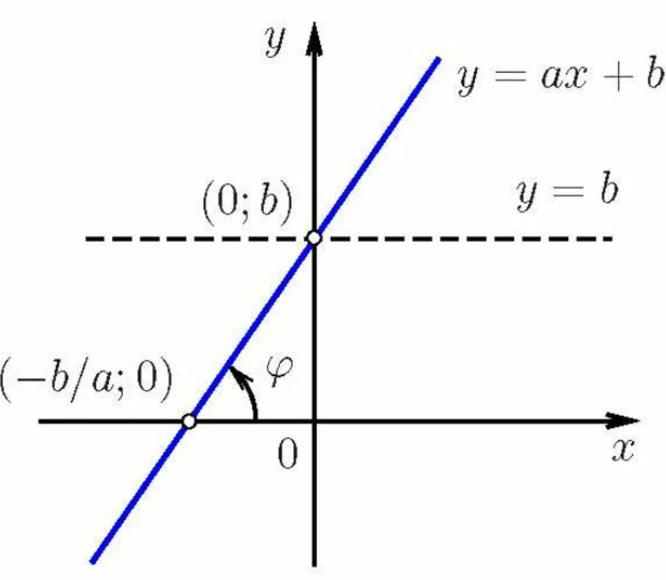
\includegraphics[width=4.42454in,height=3.8532in]{derivate-meaning-ru/image1.png}

Физический смысл производной функции.

Как было сказано ранее, необходимость в производных впервые появилась
из-за расчетов в кинематике.

Представим формулу \uline{равно}ускоренного движения

\[V(t) = V_{0} + at\]

Я немного перепишу выражение, чтобы проще было понять идею:

\[V(t) = at + V_{0}\]

Вид формулы для нахождения скорости очень похож на формулу, которой
задается линейная функция:

\[V(t) = at + \ V_{0}\ это\ как\ f(x) = kx + l\]

Откуда смело можно утверждать следующее:

Движение равноускоренное, потому что ускорение (а) не меняется. А
доказать это можно, используя смысл производной:

\(V^{'}(t) = {a(t) = (V}_{0} + at)' =\)\emph{a}

И на самом деле из формулы видно, что ускорение в зависимости от времени
не изменяется. Отсюда можно смело сказать, что:

\uline{Физический (механический) смысл производной} состоит в том, что
\uline{производная от функции расстояния}, которое прошло тело
\uline{равняется скорости движения} некоторого тела по траектории в
момент времени, и \uline{производная скорости} движения тела
\uline{равняется ускорению} этого тела

Чтобы считать производные известных элементарных функций существуют
таблицы производных, которые описывают все доказанные производные.

На следующей странице указан пример таблицы производных

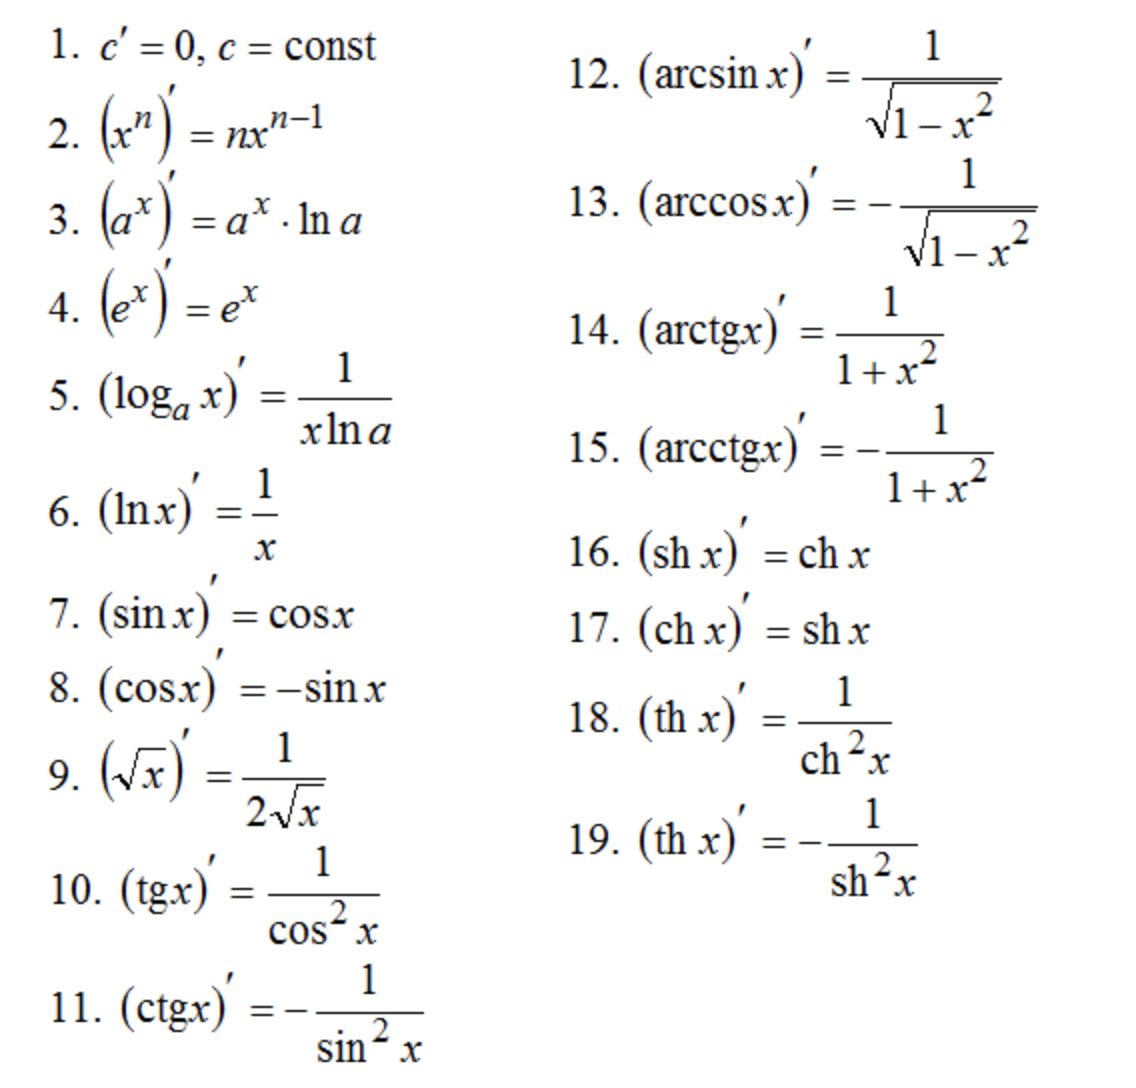
\includegraphics[width=6.49653in,height=6.22431in]{derivate-meaning-ru/image2.png}

\end{document}
